\documentclass[10pt, a4paper]{beamer}
\usetheme{Hannover}
\usecolortheme{sidebartab}
\usepackage{graphicx}
\usepackage{subcaption}
\usepackage{movie15}

\begin{document}
	\setbeamertemplate{sidebar left}{}
	\title{Progress Presentation-II}
	\subtitle{e-Yantra Summer Intership-2016 \\ \textit{Automatic Theme Evaluation From Videos}}
	\author{Raj Krishna Srivastava\\Keshav Bihani\\ {    \textbf{Mentor: Khalid Waseem}}}
	\institute{IIT Bombay}
	\date{\today}
	%\addtobeamertemplate{sidebar left}{}{\includegraphics[scale = 0.3]{logowithtext.png}}
	\frame{\titlepage}

\setbeamertemplate{sidebar left}[sidebar theme]
\section{Overview of Project}
\begin{frame}{\begin{center}
			Overview of Project
		\end{center}}\vspace{-2cm}
	\begin{itemize}
		\item \textbf{Project Name:}Automatic Theme Evaluation from Videos
		\item \textbf{Objective:}
		\begin{itemize}
			\item Automatic evaluation of black/white following robot from videos.
			\item Automatic evaluation of Puzzle Solver theme from videos.
		\end{itemize}
		\item \textbf{Deliverables:}
				\begin{itemize}
					\item Matlab code for automatic evaluation of black/white line following robot from video.
					\item Matlab code for automatic evaluation of Puzzle Solver Theme.
					\item Reports and results.
				\end{itemize}
	\end{itemize}
\end{frame}

\section{Overview of Task}
\begin{frame}{\begin{center}
			Overview of Task
		\end{center}}\vspace{-2cm}
	\begin{tabular}{|l|l|l|l|l|}
		\hline
		\textbf{Key Tasks} & \textbf{Status} & \textbf{Deadline}\\
		\hline
		Corner Detection & Accomplished & -\\
		\hline
		Object Detection for tracking & Accomplished & - \\
		\hline
		Homography & Accomplished & - \\
		\hline
		Path Evaluation(Predefined Path) & Accomplished & -\\
		\hline
		Integrating above tasks & Accomplished& 15 June\\
		\hline
		Automatic Path Evaluation& Accomplished & 22 June \\
		\hline
		Detecting picking via buzzer and led& Accomplished & 28 June \\
		\hline
		Deciding marking scheme & Pending & 30 June\\
		\hline
		Documentation and reports & Pending & 05 July\\
		\hline		
	\end{tabular}
\end{frame}

\section{Analysis of Task Accomplised}
\begin{frame}{\begin{center}
Analysis of Task Accomplised
		\end{center}}\vspace{-2cm}
	\begin{itemize}
		\item {Integration of corner detection and homography\\ with object tracking algorithm through mean-shift.}
		\item {Sound Processing to identify buzzer beep.}
		\item {Path Evaluation(Predefined Path)\\}
		\begin{itemize}
			\item {Object Tracking using Mean Shift Algorithm\\}
			\item {Calcuation of deviation from specified path.}
		\end{itemize}
	\end{itemize}
\end{frame}

\section{Sound Processing.}
\begin{frame}{\begin{center}
Sound Processing.
		\end{center}}\vspace{-1 cm}
		The task was to identify buzzer beep from various other sounds in the video and record the time frame of beeps.
		\begin{figure}[h!]
			\begin{subfigure}{0.4\textwidth}
				\includegraphics[width=0.8\linewidth, height=3.8cm]{input.jpg}
				\caption{Input}
			\end{subfigure}
			\begin{subfigure}{0.4\textwidth}
				\includegraphics[width=0.8\linewidth, height=3.8cm]{output.jpg}
				\caption{Output}
			\end{subfigure}
		\end{figure}	
\end{frame}

\begin{frame}
	\textbf{Techniques Employed}
	\begin{itemize}
		\item {Time- Domain Analysis}\\
		\begin{itemize}
			\item {Succesful in videos which were shot in predominantly quiet environment.}
			\item{Failed miserably where there were even small noise or disturbances.}
		\end{itemize}
		\item {Frequency- Domain Analysis}\\
		\begin{itemize}
			\item {Fourier Transform of time domain gives us the required Frequency Domain of the signal.}
			\item{Immune to outside noise and worked very well.}
			\item{All robots had frequency between 2.7kHz to 3 kHz.}
		\end{itemize}
	\end{itemize}
\end{frame}

\begin{frame}
		\textbf{Intermediate Stages}
		\begin{figure}[h!]
			\begin{subfigure}{0.4\textwidth}
				\includegraphics[width=0.6\linewidth, height=2.4cm]{Filtering/2.jpg}
				\caption{Image after thresholding}
			\end{subfigure}
			\begin{subfigure}{0.4\textwidth}
				\includegraphics[width=0.6\linewidth, height=2.4cm]{Filtering/3.jpg}
				\caption{Image after filling holes}
			\end{subfigure}
			\begin{subfigure}{0.4\textwidth}
				\includegraphics[width=0.6\linewidth, height=2.4cm]{Filtering/4.jpg} 
				\caption{Image after erosion and dilation}
			\end{subfigure}
			\begin{subfigure}{0.4\textwidth}
				\includegraphics[width=0.6\linewidth, height=2.4cm]{Filtering/5.jpg}
				\caption{Image after selecting the patch with max. area}
			\end{subfigure}
		\end{figure}
\end{frame}

\begin{frame}
	\textbf{Challenges}
	\begin{itemize}
		\item {Designing of filters was bit of a task.}\\
		Choosing the order of filter and determining the type of filter as in butter filter or various other filters offered by matlab was quiet confusing and challenging.
	\end{itemize}
	
\end{frame}

\begin{frame}
	\textbf{Robot Detection}
	\textbf{Techniques}
	\begin{itemize}
		\item {Using filtering and masking.}
			\begin{figure}[h!]
				\begin{subfigure}{0.4\textwidth}
					\includegraphics[width=0.6\linewidth, height=2cm]{Filtering/objectdetection/1.jpg}
					\caption{Original Image}
				\end{subfigure}
				\begin{subfigure}{0.4\textwidth}
					\includegraphics[width=0.6\linewidth, height=2cm]{Filtering/objectdetection/2.jpg}
					\caption{Image after filtering}
				\end{subfigure}
				\begin{subfigure}{0.4\textwidth}
					\includegraphics[width=0.6\linewidth, height=2cm]{Filtering/objectdetection/3.jpg} 
					\caption{Robot Identified}
				\end{subfigure}
			\end{figure}
		\item {Machine Learning.}
	\end{itemize}	
\end{frame}
\begin{frame}
	\textbf{Corner Detection}
	\textbf{Techniques}
	\begin{itemize}
		\item {Using Harris-Corner Detection.}\\
		\begin{itemize}
			\item Not sure that it will only give four corners.
		\end{itemize}
		\item {Detection using polar-coordinates.}
		\begin{itemize}
			\item Not efficient method and does not give desired output for our images.
		\end{itemize}
		\item {By dot product of two vectors.}
		\begin{itemize}
			\item Absurd results since the edges of the masked images are not smooth enough.
		\end{itemize}
		\item {Using markers.}
		\begin{itemize}
			\item Results somewhat accurate and meaningful.
		\end{itemize}
	\end{itemize}	
\end{frame}
\begin{frame}
	\textbf{Results after using methods with marker}
	\begin{figure}[h!]
		\begin{subfigure}{0.4\textwidth}
			\includegraphics[width=1\linewidth, height=5cm]{Filtering/cornerdetection/1.jpg}
			\caption{Input}
		\end{subfigure}
		\begin{subfigure}{0.4\textwidth}
			\includegraphics[width=1\linewidth, height=5cm]{Filtering/cornerdetection/2.jpg}
			\caption{Output}
		\end{subfigure}
	\end{figure}	
\end{frame}

\begin{frame}
	\textbf{Challenges}
	\begin{itemize}
		\item {Due to varying lighting conditions.}
	\end{itemize}
	\begin{figure}[h!]
		\begin{subfigure}{0.4\textwidth}
			\includegraphics[width=1\linewidth, height=4cm]{Filtering/challenges/1.jpg}
			\caption{Input}
		\end{subfigure}
		\begin{subfigure}{0.4\textwidth}
			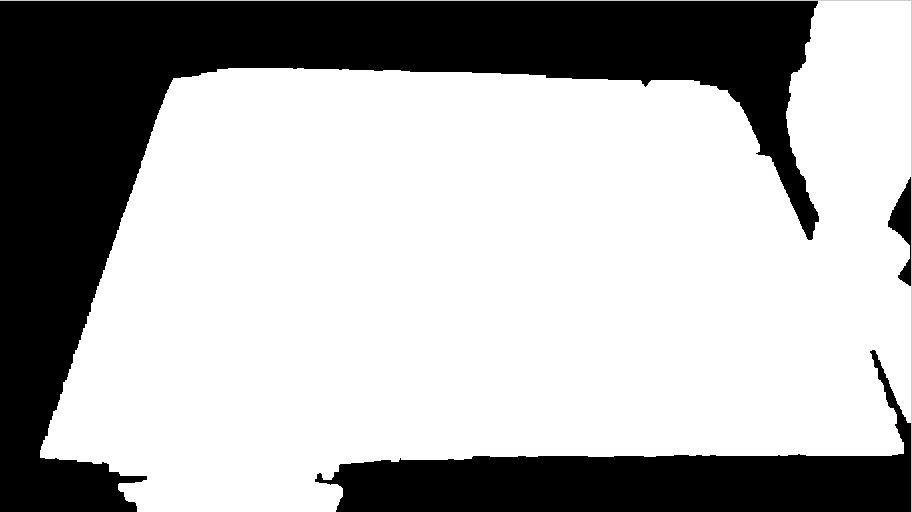
\includegraphics[width=1\linewidth, height=4cm]{Filtering/challenges/11.jpg}
			\caption{Output}
		\end{subfigure}
	\end{figure}	
\end{frame}
\begin{frame}
	\begin{figure}[h!]
		\begin{subfigure}{0.4\textwidth}
			\includegraphics[width=1\linewidth, height=4cm]{Filtering/challenges/3.jpg}
			\caption{Input}
		\end{subfigure}
		\begin{subfigure}{0.4\textwidth}
			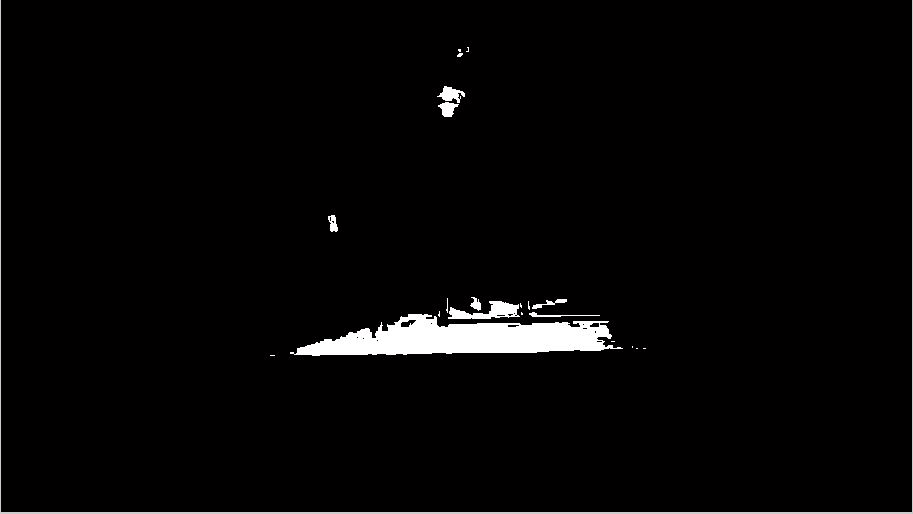
\includegraphics[width=1\linewidth, height=4cm]{Filtering/challenges/33.jpg}
			\caption{Output}
		\end{subfigure}
	\end{figure}	
\end{frame}

\begin{frame}
	\begin{itemize}
		\item {Due to kinds of surfaces.}
	\end{itemize}
	
	\begin{figure}[h!]
		\begin{subfigure}{0.4\textwidth}
			\includegraphics[width=1\linewidth, height=4cm]{Filtering/challenges/2.jpg}
			\caption{Input}
		\end{subfigure}
		\begin{subfigure}{0.4\textwidth}
			
\includegraphics[width=1\linewidth, height=4cm]{Filtering/challenges/22.jpg}
			\caption{Output}
		\end{subfigure}
	\end{figure}	
\end{frame}

\section{Homography}
\begin{frame}{\begin{center}
			Homography
		\end{center}}\vspace{-1 cm}
		Now the next big challenge was to bring all the videos taken from different angles to a similar viewing angle so that evaluation is easier. This is done by method known as homography. For instance we have these images for theme Puzzle Solver 2 taken by different teams.
		\begin{figure}[h!]
			\includegraphics[scale=0.1]{Homography/1.jpg}
			\centering
			\caption{Testing Purpose}
		\end{figure}	
		
\end{frame}

\begin{frame}
	\begin{figure}[h!]
		\includegraphics[width=1\linewidth, height=8cm]{Homography/2.jpg}
		\centering
		\caption{Testing Purpose}
	\end{figure}	
\end{frame}
\begin{frame}
	\begin{figure}[h!]
		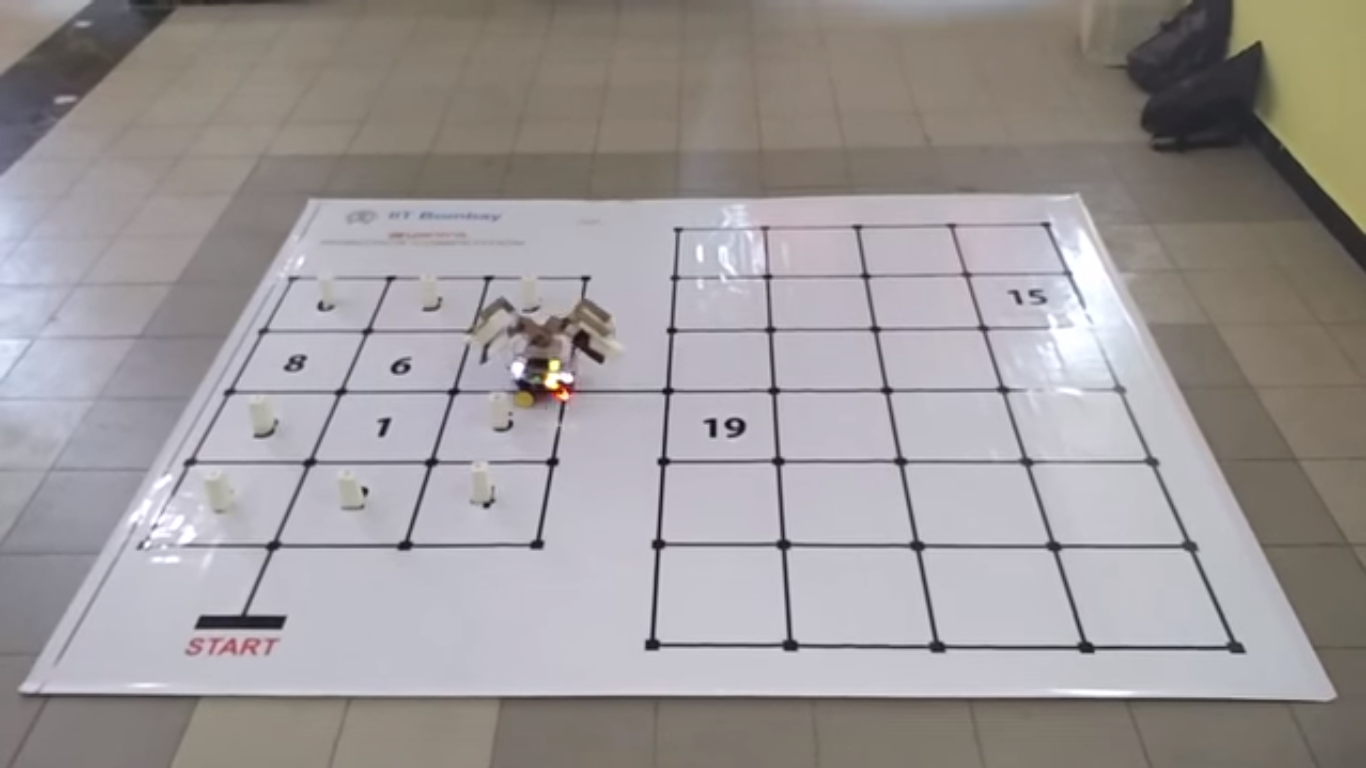
\includegraphics[width=1\linewidth, height=8cm]{Homography/3.png}
		\centering
		\caption{Team:PS2\#1096}
	\end{figure}	
\end{frame}
\begin{frame}
	\begin{figure}[h!]
		\includegraphics[width=1\linewidth, height=8cm]{Homography/4.jpg}
		\centering
		\caption{Team:PS2\#1504}
	\end{figure}	
\end{frame}
\begin{frame}
	\begin{figure}[h!]
		\includegraphics[width=1\linewidth, height=8cm]{Homography/5.png}
		\centering
		\caption{5}
	\end{figure}	
\end{frame}
\begin{frame}
	{\begin{center}
			Result after homography.
		\end{center}}\vspace{-1 cm}
	\begin{figure}[h!]
		\begin{subfigure}{0.4\textwidth}
			\includegraphics[width=1\linewidth, height=5cm]{Homography/homographed/1.jpg}
			\caption{Input}
		\end{subfigure}
		\begin{subfigure}{0.4\textwidth}
			\includegraphics[width=1\linewidth, height=5cm]{Homography/homographed/2.jpg}
			\caption{Output}
		\end{subfigure}
	\end{figure}	
\end{frame}

\section{Path Evaluation}
\begin{frame}{\begin{center}
			Path Evaluation
		\end{center}}\vspace{-2cm}
	\begin{figure}[ht]
		\includemovie[poster,text={\small(Loading Video...)}]{6cm}{4cm}{movie.mp4}
	\end{figure}
\end{frame}

\section{Thank You}
\begin{frame}{\begin{center}
Thank You.
		\end{center}}\vspace{-2cm}
	\centering THANK YOU !!!\\
	. .\\
	 U 
\end{frame}
\end{document}
